\section{Technical Background}

\subsection{Machine learning}
Machine learning is a subset of artificial intelligence that uses statistical inference to adapt responses based on previous and new knowledge. This is a very powerful type of program as it provides adaptability at no code architecture change, however, these systems improve drastically the more data it has available and analyzed \cite{IBM-MachineLearningTypes}.

\begin{figure}[h]
	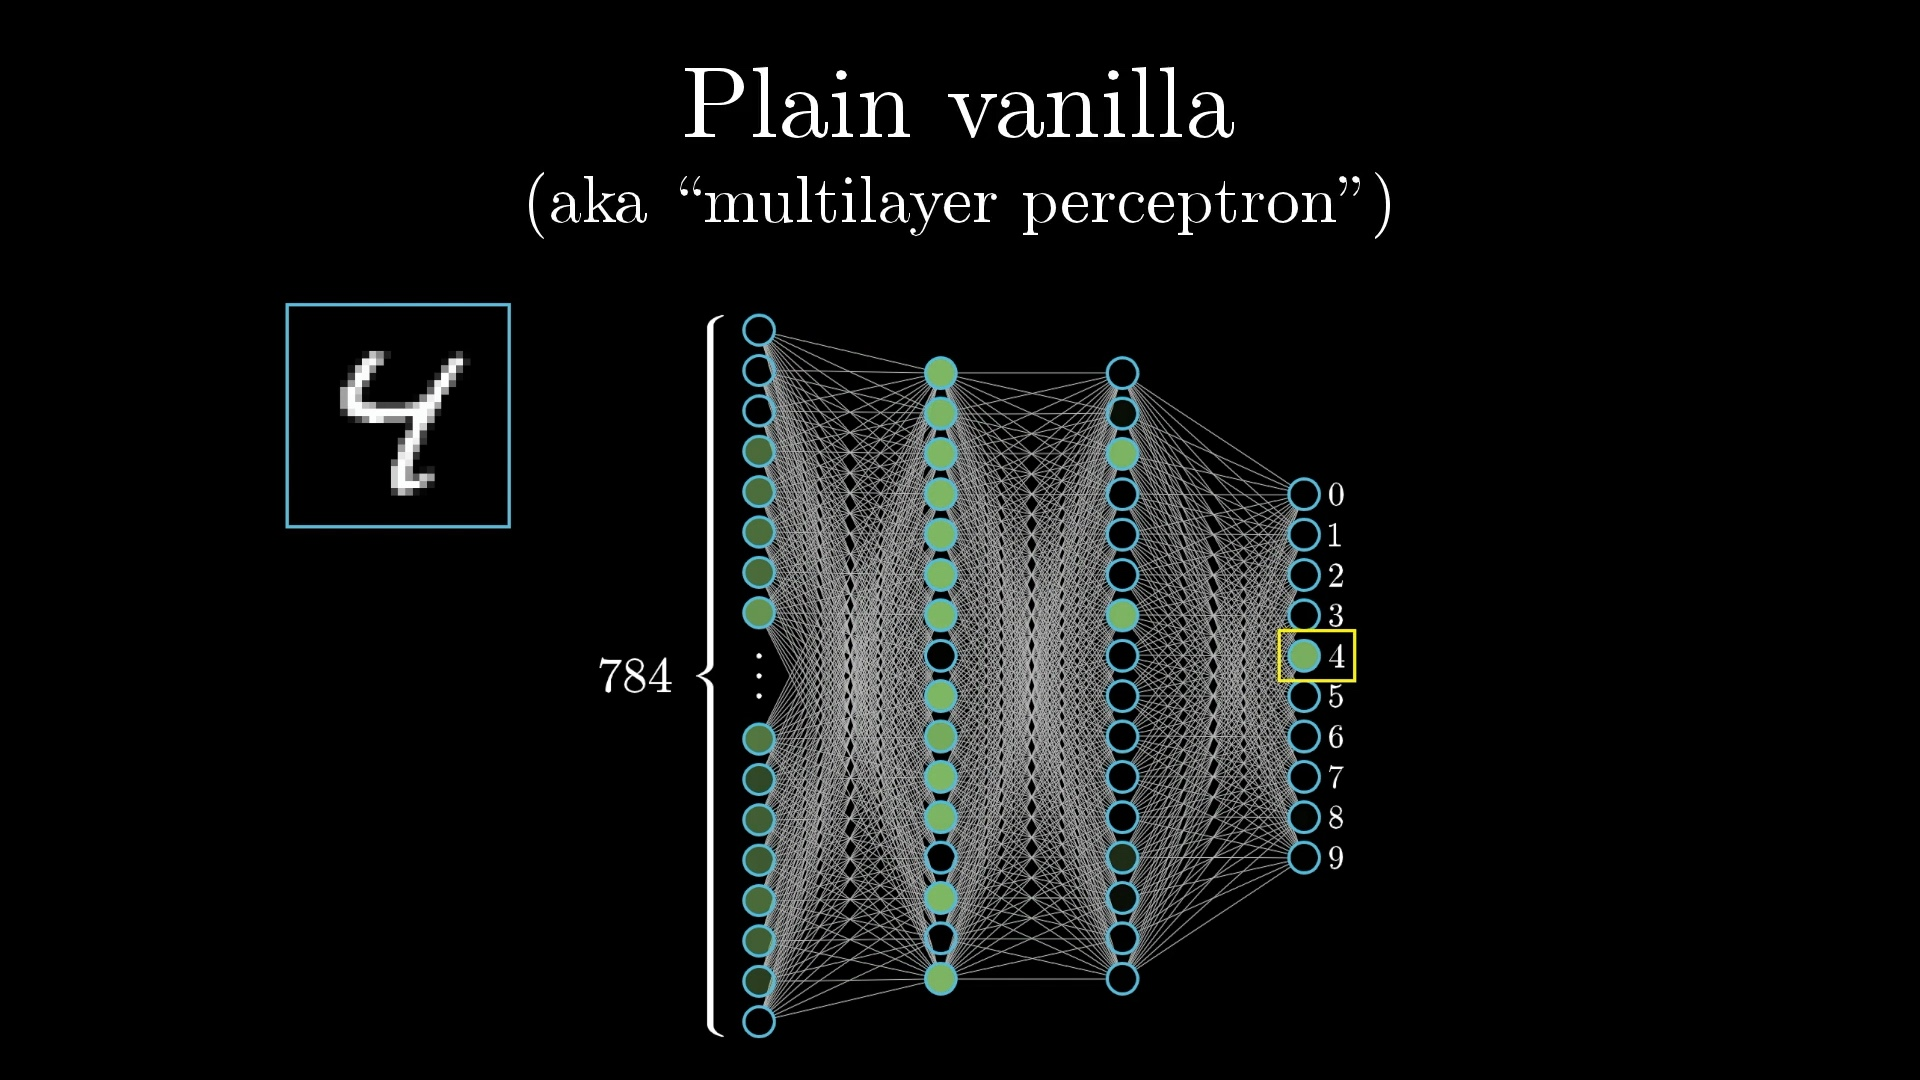
\includegraphics[width=\columnwidth]{plain-vanilla.jpg}
	\caption{Neural network made to recognize numbers 0 to 9 on a 28 by 28 grid \cite{what-is-a-neural-network}.}
	\label{Neural-Network}
\end{figure}

Models work via the implementation of neural networks. A neural network is composed of \textit{neurons}, which are simply just a number that represents the presence of a component in the data (the circles in the image \ref{Neural-Network}). A vector of neurons represents a layer, this is used to represent different components of the data. Neural networks are normally composed of several layers each neuron connected to another via weights (the lines in image \ref{Neural-Network}). This allows the model to encode the activation of a neuron based on a linear combination of the weights and neurons of the previous layer. In the image \ref{Neural-Network} the activation is represented by how green each circle is. Each layer encodes different sets of properties about the data, in the case of figure \ref{Neural-Network} the first layer represents how bright each pixel is while the next one represents relationships in the distributions. The first layer is one of the few layers that can be explicitly linked to the data as the activation is entirely determined by the model maker. This is because these linear combinations can be fine tuned with a bias term to ensure that the model produces better results \cite{what-is-a-neural-network}.

\begin{figure}[h]
	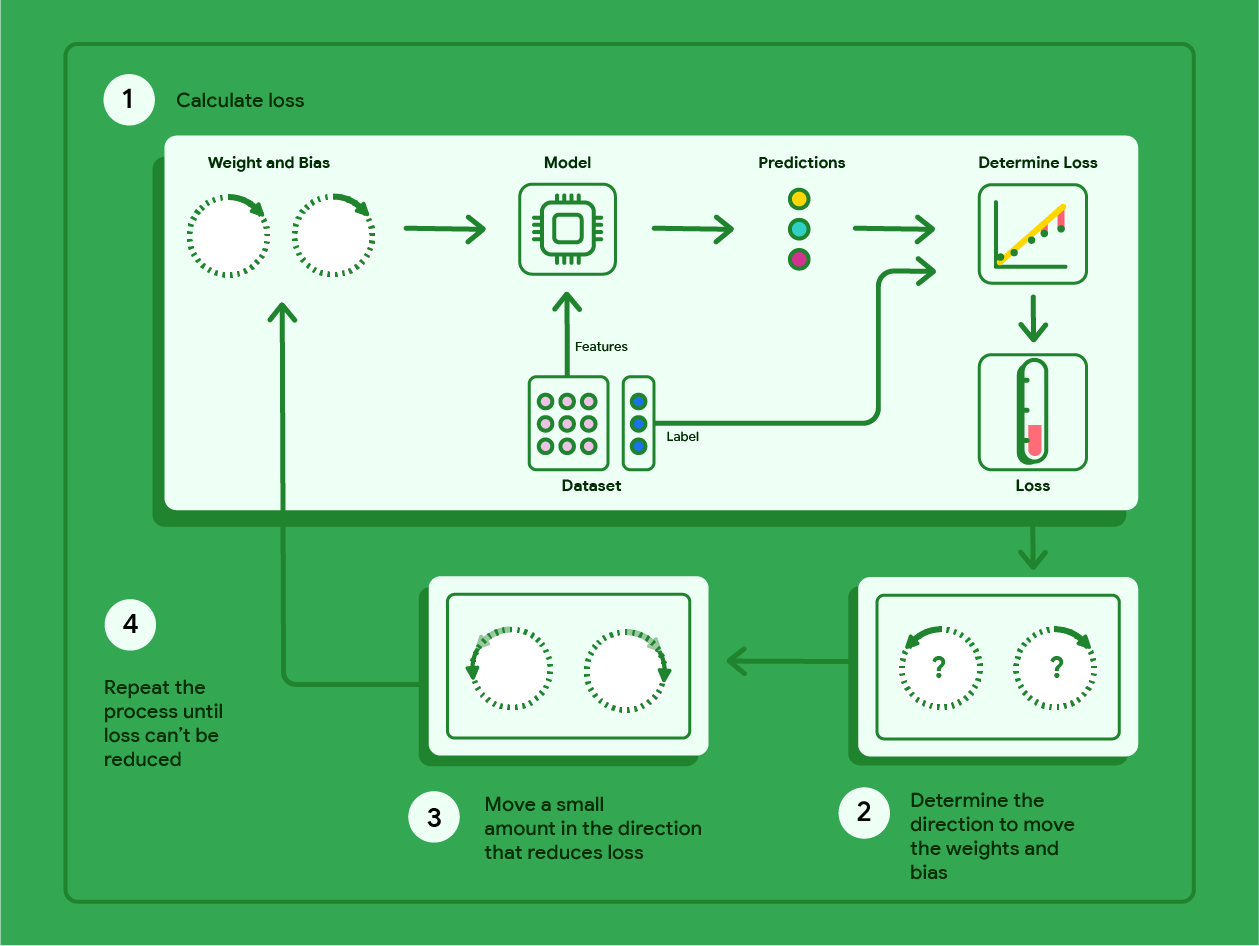
\includegraphics[width=\columnwidth]{gradient-descent.png}
	\caption{The model training pipeline \cite{gradient-descent}}
	\label{Gradient-Descent}
\end{figure}

The training process for a model involves utilizing data that is labelled to be the right response and iteratively improving all of the model's weights and biases (denoted by $\vec{w}$). This process of improvement utilizes cost function and gradient descent. The cost function ($\epsilon$) describes the error of the current model based on the given parameters, this error is normally averaged to improve across all input types instead of only one \cite{gradient-descent}. Gradient descent is an iterative optimization method defined as such:

\newcommand{\pardev}[2]{\frac{\partial #1}{\partial #2}}

$$
	\vec{w'} = \vec{w} + \gamma \begin{bmatrix}
		\pardev{\epsilon}{w_1} \\
		\vdots                 \\
		\pardev{\epsilon}{w_n} \\
	\end{bmatrix}
$$

This method is used for steps 2 and 3 in figure \ref{Gradient-Descent} as it will calculate the direction to move the weights and biases and move there. This process is repeated until the change in error between iterations is less than desired \cite{gradient-descent}. While this only adjusts the weights, there still needs to be a process of back-propagation. This involved finding which parameters affect the output the most and then adjusting the values to cover the edge cases left after the gradient descent is done \footnote{The math of this algorithm is more complex therefore it will not be explored in depth for this essay} \cite{backpropagation}.

\subsection{Large Language Models}
A large language model is a form of generative AI which utilizes the encoded relationships from machine learning to produce new content based on a word input.

\subsection{Architecture of GenAI coding tools}
When utilizing generative AI in the context of a software project, there are additional considerations that must be met to meet the desired output. To better understand this fine tuning, this essay will focus on Claude Code's approach as a case study.

\begin{figure}[h]
	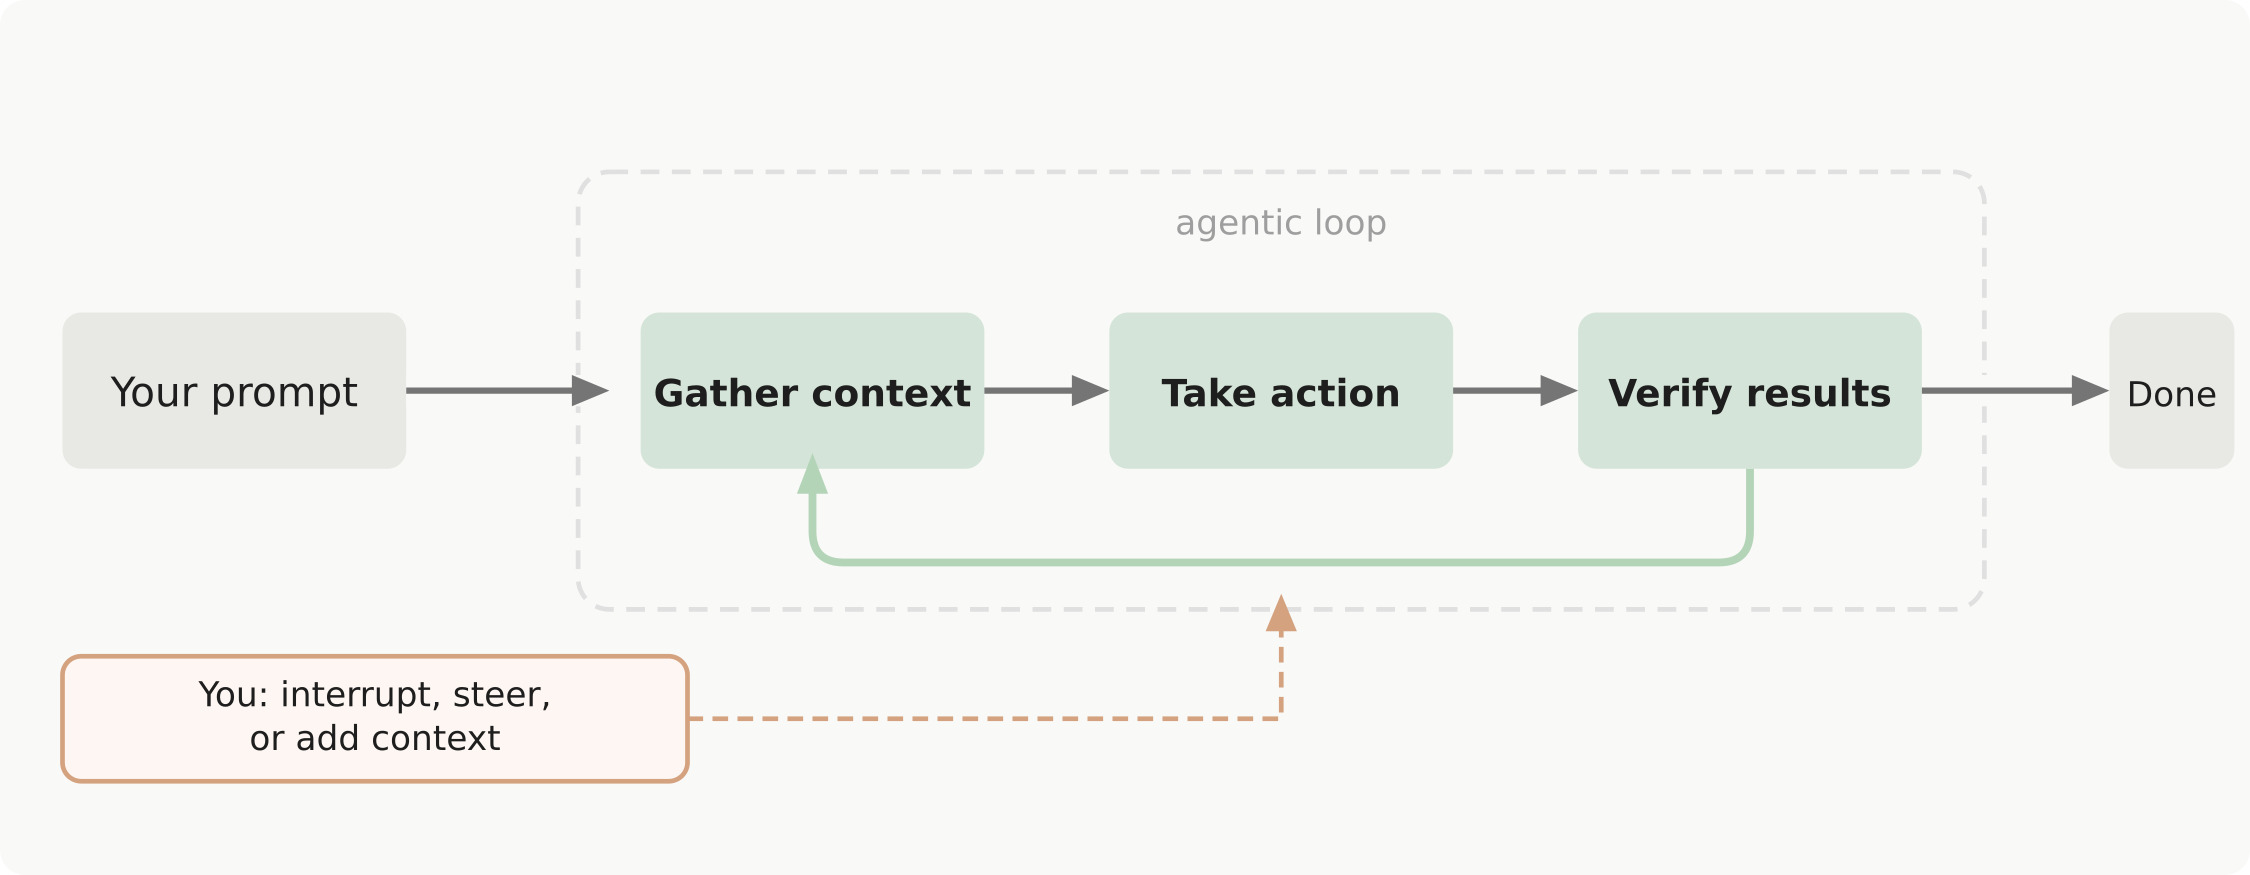
\includegraphics[width=\columnwidth]{agentic-loop.jpg}
	\caption{Claude Code's prompt processing architecture \cite{claude}}
	\label{Claude-Agentic-Loop}
\end{figure}

When a developer prompts a Claude Code, the tool will start by gathering context of the problem. This involves analyzing the codebase for relevant symbols and classes that are needed to complete the required prompt. Then the tool will execute actions such as generating text or code. Lastly, because Claude has permissions to interact with the terminal, it will try to verify the results by either compiling the code, running the code and verifying any output produced by the program \cite{claude}.

While not all developers directly allow GenAI tools to access their codebase, this is the most effective at producing responses as it is able to gather more information and test the generated content.
